\section{Dokumentace}
\label{sc:documentation}
Dokumentace se dělí na dvě části, a to technická dokumentace pro vývojáře a uživatelská pro nového uživatele. Uživatelská dokumentace je potřeba pro komplexní systémy, pro aplikace které mají zaujmout a udžet uživatele je většinou spíše na škodu. Uživatel si totiž raději zvolí intuitivní alternativu, než aby četl návod na použití, a z~toho důvodu tato aplikace místo uživatelské dokumentace cílí na co nejlepší přehlednost a intuitivnost.

Technická dokumentace na druhou stranu je nezbytná pro další vývoj aplikace. Taková dokumentace musí přehledně, stručně ale výstižně popsat architekturu a jednotlivé části aplikace. V~rámci této práce se jedná o~dva konkrétní typy dokumentace. První typ je pomocí \nameref{ss:storybook}. Ke všem komponentám, které jsou použité na více místech existuje story soubor, který popisuje jednotlivé možnosti komponenty závisející na vstupních parametrech komponenty. Tento přístup zajišťuje hlavně to, že komponenta nemá žádné vedlejší efekty, tedy neovlivňuje ani není ovlivněna jiné komponenty. Druhý typ dokumentace je automaticky generovaná pomocí nástroje \href{https://typedoc.org/}{\emph{TypeDoc}}, který projde všechny typescript soubory a z~validních \href{https://jsdoc.app/}{\emph{JSDoc}} komentářů vytvoří dokumentaci. Tento nástroj je podobný například nástroji \href{http://www.doxygen.nl/}{\emph{doxygen}}. Aby TypeDoc fungoval správně s~monorepozitáři, tak je zapotřebí použít plugin \emph{typedoc-plugin-external-module-map}. Tento plugin bohužel nefungoval s~novou verzí TypeDocu a staré verze TypeDocu nefungovali s~novou verzí Yarnu. Naštěstí oprava byla triviální a díky rychlému schválení pull requestu \footnote{https://github.com/asgerjensen/typedoc-plugin-external-module-map/pull/9} šlo tento plugin použít. Příklad validního JSDoc komentáře je vídět na obrázku \ref{code:jsdoc} a podle toho vygenerovaná dokumentace na obrázku \cite{fig:documentation_example}.

\begin{figure}[h!]
    \centering
    \begin{minted}{typescript}
/**
 * Update {@link Author}
 *
 * @param fieldsToUpdate Field to be updated
 * @returns New updated {@link Author} object
 */
update(fieldsToUpdate: Partial<Omit<Author, 'id'>>): Author {
    const newEntity: Author = { ...this._entity, ...fieldsToUpdate };
    return newEntity;
}
    \end{minted}
    \caption{JSDoc ukázka, metoda v~AuthorInteractor}
    \label{code:jsdoc}
\end{figure}

\begin{figure}[h!]
    \centering
    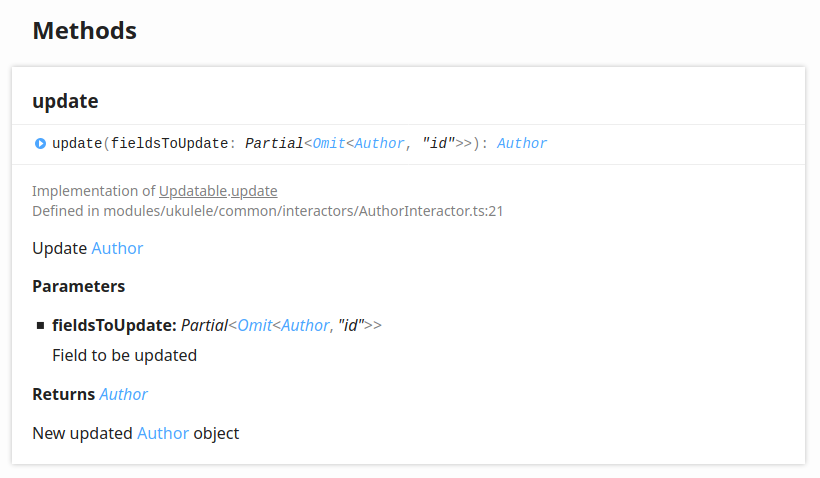
\includegraphics[width=0.9\textwidth]{assets/author_documentation.png}
    \caption{Ukázka vygenerované dokumentace}
    \label{fig:documentation_example}
\end{figure}
